%%%%%%%%%%%%%%%%%%%%%%%%%%%%%%%%%%%%%%%%%%%%%%%%%%%%%%%%%%%%%%%%%%%
% Chapter2: Related Work
%%%%%%%%%%%%%%%%%%%%%%%%%%%%%%%%%%%%%%%%%%%%%%%%%%%%%%%%%%%%%%%%%%%

\chapter{Related Works}
\label{chap:related_work}

% % tôi sẽ chuyển cái này thành 1 idea để viết phương pháp
% % kiểu: Lấy ý tưởng từ ensemble model này kia
% \section{Ensemble models}

\section{Deep feature-based approach}

\subsection{Convolutional neural network}

\subsection{Recurrent Neural Network}

\subsection{Long Short-Term Memory}

\section{Frequency decomposition approach}

\subsection{A transformer-based method}

\subsection{NHITS}

% Neural Hierarchical Interpolation for Time Series Forecasting (\verb|NHITS|) \cite{challu2023nhits} được thiết kế để hướng đến việc dự đoán một long-horizon time-series data bằng cách phân rã tín hiệu đầu vào thành các dải tần số riêng biệt. Cấu trúc của \verb|NHITS| bao gồm $S$ stack, mỗi stack bao gồm $B$ block nối tiếp nhau. Tại mỗi block, một Multi-layer perceptron (\verb|MLP|) sử dụng dữ liệu lịch sử để dự đoán chính nó và dữ liệu tương lai (see figure \ref{fig:nhits}).

Neural Hierarchical Interpolation for Time Series Forecasting (\verb|NHITS|) \cite{challu2023nhits} is designed to target the prediction of long-horizon time-series data by decomposing the input signal into discrete frequency bands. The structure of \verb|NHITS| consists of $S$ stacks, each stack consisting of $B$ consecutive blocks. At each block, a Multi-layer perceptron (\verb|MLP|) uses historical data to predict itself and future data (see figure \ref{fig:nhits}).

\begin{figure}[H]
    \centering
    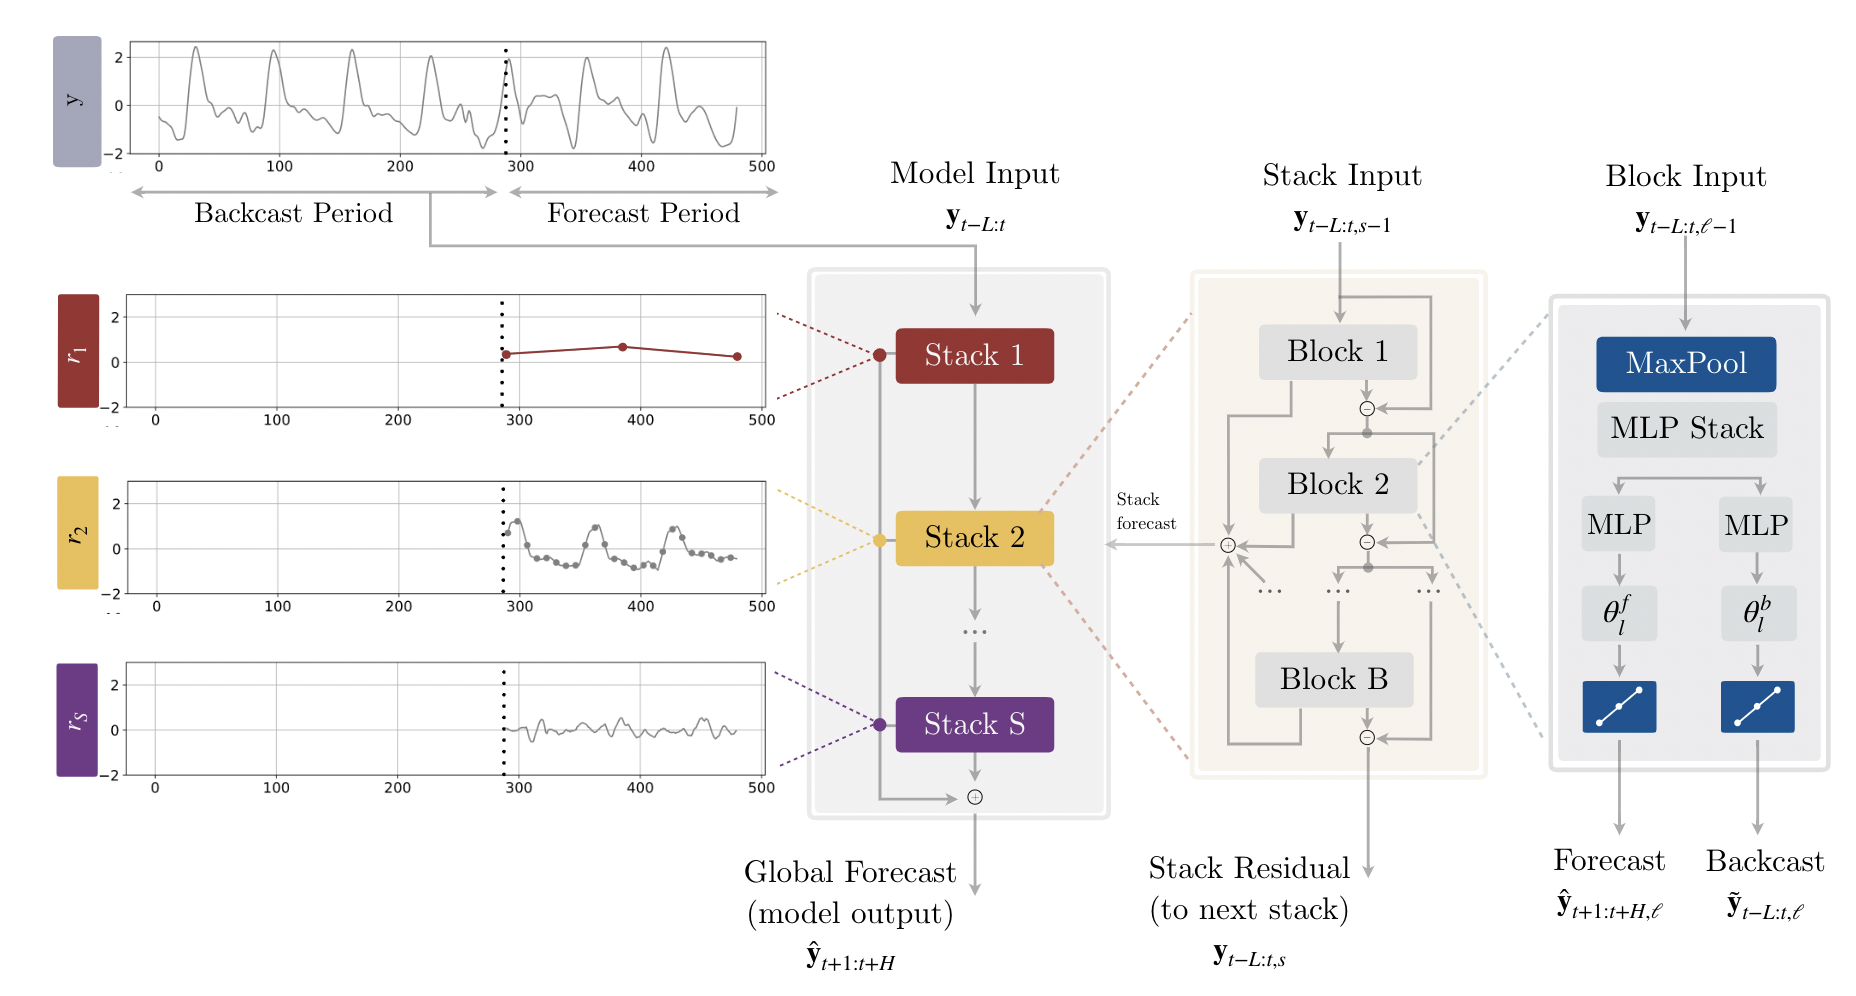
\includegraphics[width=\textwidth]{nhits-arch.png}
    \cprotect\caption{\verb|NHITS| architecture \cite{challu2023nhits}.}
    \label{fig:nhits}
\end{figure}

% Cụ thể, tại block $l$, với $L$ mẫu dữ liệu quá khứ ($\mathbf{y}_{t-L:t, l-1}$), một \verb|MLP| sẽ sử dụng lần lượt ba kỹ thuật Multi-rate signal sampling, Non-linear regression, và Hierarchical interpolation để hồi quy dữ liệu quá khứ và dự đoán dữ liệu tương lai.

Specifically, at block $l$, with $L$ historical samples ($\mathbf{y}_{t-L:t, l-1}$), an \verb|MLP| use three techniques, Multi-rate signal sampling, Non-linear regression, and Hierarchical interpolation, respectively, to regress past data and predict future data.

% \textbf{Multi-rate signal sampling}. \verb|MaxPool| layer với kernel size $l$ nén dữ liệu ban đầu vào $\mathbf{y}_{t-L:t, l}^{(p)}$ (equation \ref{eq:maxPool}). Khi $k_l$ lớn, lượng dữ liệu được xét trong một cửa sổ trượt lớn, mạng sẽ chú ý đến các sóng tín hiệu với bước sóng dài (tần số thấp). Khi $k_l$ nhỏ, các đặc trưng thu được là của các bước sóng nhỏ (tần số cao). Bằng việc sử dụng lớp \verb|MaxPool|, các \verb|MLP| sẽ có khả năng làm việc trên một dải tần nhất định, giúp tăng hiệu quả của việc phân rã tần số. Không chỉ dừng lại ở việc phân tách dải tần, \verb|MaxPool| về cơ bản làm giảm kích thước của tín hiệu đầu vào, giúp tiết kiệm bộ nhớ trong quá trình training và inference.

\textbf{Multi-rate signal sampling}. \verb|MaxPool| layer with kernel size $l$ compresses the original data into $\mathbf{y}_{t-L:t, l}^{(p)}$ (equation \ref{eq:maxPool}). When $k_l$ is large, the amount of data considered in a sliding window is also large, the network will pay more attention to input signal with long wavelengths (low frequencies). When $k_l$ is small, the obtained features are of short wavelengths (high frequencies). By using \verb|MaxPool| layer, \verb|MLP| will be able to work on a certain frequency band, which helps to increase the efficiency of frequency decomposition. Not only stopping at frequency band decomposition, \verb|MaxPool| essentially reduces the size of the input signal, helping to save memory during training and inference.

\begin{align}
    \mathbf{y}_{t-L:t, l}^{(p)} = \mathbf{MaxPool}\left( \mathbf{y}_{t-L:t, l-1}, k_l \right)
    \label{eq:maxPool}
\end{align}

% \textbf{Non-linear regression}. Sau khi nén dữ liệu, \verb|NHITS| tiến hành học các hệ số nội suy bằng các perceptron layer xếp chồng với hàm kích hoạt phi tuyến (\verb|FullyConnected|). Mục tiêu của \verb|FullyConnected| là tạo ra các vector $\mathbf{\theta}_l^f, \mathbf{\theta}_l^b$ (equation \ref{eq:non_linear}). Đây là hai vector nội suy forecast và backcast, được dùng để tổng hợp các giá trị đầu ra của block $l$ bằng hàm nội suy $g(\cdot)$. Trong đó, $\mathbf{\theta}_l^f$ được dùng để dự báo các giá trị tương lai còn $\mathbf{\theta}_l^b$ được dùng để hồi quy các giá trị input.

\textbf{Non-linear regression}. After compressing the data, \verb|NHITS| learns the interpolation coefficients using stacked perceptron layers with a nonlinear activation function (\verb|FullyConnected|). The goal of \verb|FullyConnected| is to generate the vectors $\mathbf{\theta}_l^f, \mathbf{\theta}_l^b$ (equation \ref{eq:non_linear}). These are the two interpolation vectors forecast and backcast, which are used to aggregate the output values of block $l$ using the interpolation function $g(\cdot)$. In which, $\mathbf{\theta}_l^f$ is used to forecast future values and $\mathbf{\theta}_l^b$ is used to regress the input values.

\begin{align}
    \mathbf{\theta}_l^b &= \mathbf{FullyConnected}^b \left( \mathbf{y}_{t-L:t, l}^{(p)} \right)\\
    \mathbf{\theta}_l^f &= \mathbf{FullyConnected}^f \left( \mathbf{y}_{t-L:t, l}^{(p)} \right)\\
    \label{eq:non_linear}
\end{align}

% \textbf{Hierarchical interpolation}. Để dự đoán $H$ giá trị tương lai, một mạng neural thông thường phải thiết kế lại số neuron đầu ra. Đôi với mô hình transformer, muốn tăng số mẫu đầu ra, cần phải tăng số mẫu đầu vào để các layer cross-attention hoạt động hiệu quả. Điều này khiến cho quá trình huấn luyện truyền thống tiêu tốn rất nhiều tài nguyên khi có nhu cầu dự đoán $H$ lớn. \verb|NHITS| giải quyết vấn đề này bằng cách sử dụng phương trình nội suy với các hệ số nội suy đã được chuẩn bị trước ở bước \textbf{Non-linear regression} (equation \ref{eq:interpolation}). Số chiều của các hệ số nội suy trong mỗi stack được quy định bởi expressiveness ratio $r_l$: $\left| \theta_l \right| =  \left \lceil r_l H \right \rceil$. Thông thường, expressiveness ratio sẽ rất nhỏ ở các stack đầu tiên và tăng dần về cuối. Theo đó, các stack có thể mô phỏng lại các tần số từ thấp đến cao. Ngoài ra, bằng việc sử dụng hàm nội suy, \verb|NHITS| không cần quá nhiều phần cứng để huấn luyện mạng neural trong trường hợp $H$ lớn.

\textbf{Hierarchical interpolation}. To forecast $H$ future values, a conventional neural network must redesign the number of output neurons. For transformer models, to increase the number of output samples, it is necessary to increase the number of input samples so that the cross-attention layers can work effectively. This makes the traditional training process very resource-consuming when there is a need to predict large $H$. \verb|NHITS| solves this problem by using an interpolation equation with pre-prepared interpolation coefficients in the \textbf{Non-linear regression} step (equation \ref{eq:interpolation}). The dimensionality of the interpolation coefficients in each stack is determined by the expressiveness ratio $r_l$: $\left| \theta_l \right| = \left \lceil r_l H \right \rceil$. Typically, the expressiveness ratio will be very small in the first stacks and gradually increase towards the end. Accordingly, the stacks can simulate frequencies from low to high. In addition, by using the interpolation function, \verb|NHITS| does not require too much hardware to train the neural network in the case of large $H$.

\begin{align}
    \mathbf{\hat{y}}_{t-L:t, l} &= g\left(\mathbf{\theta}_l^b\right)\\
    \mathbf{\hat{y}}_{t+1:t+H, l} &= g\left(\mathbf{\theta}_l^f\right)
    \label{eq:interpolation}
\end{align}

% Đầu ra của block $l$ là giá trị forecast $\mathbf{\hat{y}}_{t+1:t+H, l}$ và giá trị backcast $\mathbf{\hat{y}}_{t-L:t, l}$. Input of block $l+1$ is the difference between the its backcast and its output (\ref{eq:input_l1}).

The output of block $l$ is the forecast value $\mathbf{\hat{y}}_{t+1:t+H, l}$ and the backcast value $\mathbf{\hat{y}}_{ t-L:t, l}$. Input of block $l+1$ is the difference between its backcast and its output (\ref{eq:input_l1}).

\begin{align}
    \mathbf{y}_{t-L:t, l+1} = \mathbf{y}_{t-L:t, l-1} - \mathbf{\hat{y}}_{t-L:t, l}
    \label{eq:input_l1}
\end{align}

% Tổng hợp các giá trị forecast của $B$ block như phương trình \ref{eq:sum_block}, ta được giá trị forecast của một stack. Cuối cùng, tổng hợp giá trị forecast của các stack như phương trình \ref{eq:sum_stack}, ta được giá trị forecast dự đoán của toàn mạng.

Summing the forecast values of $B$ blocks as in equation \ref{eq:sum_block}, we get the forecast value of a stack. Finally, summing the forecast values of the stacks as in equation \ref{eq:sum_stack}, we get the predicted forecast value of the entire network.

\begin{align}
    \mathbf{\hat{y}}_{t+1:t+H}^s &= \sum_{l=1}^{B}{\mathbf{\hat{y}}_{t+1:t+H, l}} \label{eq:sum_block}\\
    \mathbf{\hat{y}}_{t+1:t+H} &= \sum_{s=1}^{S}{\mathbf{\hat{y}}_{t+1:t+H}^s} \label{eq:sum_stack}
\end{align}

% Bằng cách xếp chồng các stack, stack sau nhận vào phần dư của stack trước, kiến trúc trên được kỳ vọng là sẽ phân rã dữ liệu thành các frequency bands khác nhau (weekly, daily, even hourly). Trong thực tế, \verb|NHITS| perform rất tốt đối với các bộ dữ liệu có tính chu kỳ cao như mức tiêu thụ điện, thời tiết, giao thông. Tuy nhiên, chúng tôi đang hướng đến aperiodic time-series dataset, vốn có tính chu kỳ rất thấp. Điều này gây ra khó khăn rất lớn cho \verb|NHITS|.

By concatenating stacks, each receiving the remainder of the previous stack, the above architecture is expected to decompose the data into different frequency bands (weekly, daily, even hourly). In practice, \verb|NHITS| performs very well for highly periodic datasets such as electricity consumption, weather, traffic. However, we are aiming for an aperiodic time-series dataset, which has very low, or even non-existent, periodicity. This poses a huge challenge for \verb|NHITS|.

\section{Optimization-based Meta-learning}
\label{sec:ml}

% Meta-learning (ML) là một phương pháp huấn luyện cho phép mô hình học có thể gia tăng kinh nghiệm qua việc thực hiện nhiều task khác nhau trong cùng một phân phối task. Việc này trạng bị cho mô hình học máy khả năng tổng quát hóa cao, thích ứng nhanh trên task mới chỉ sau một vài bước huấn luyện với dữ liệu huấn luyện giới hạn \cite{hospedales2021meta, vettoruzzo2024advances}. Với khả năng này, ML được sử dụng rất nhiều trong các tác vụ đòi hỏi khả năng đáp ứng của mô hình trên dữ liệu (e.g. cá nhân hóa mô hình học \cite{chen2018federated, fallah2020personalized,nguyen2022meta}, domain adaptation trong online learning \cite{hu2023meta, khoee2024domain}).

Meta-learning (ML) is a training method that allows a learning model to gain experience by performing many different tasks in the same task distribution. This equips the machine learning model with the ability to generalize highly and adapt quickly to new tasks after only a few training steps with limited training data \cite{hospedales2021meta, vettoruzzo2024advances}. With this ability, ML is widely used in tasks that require the ability to fast adapt to new data (e.g. personalization of learning models \cite{chen2018federated, fallah2020personalized,nguyen2022meta}, domain adaptation in online learning \cite{hu2023meta, khoe2024domain}).

% Đối với phương pháp huấn luyện mô hình học truyền thống, chúng ta huấn luyện mô hình dự đoán $\hat{y} = f_\theta(\mathbf{x})$ trên tập dữ liệu $\mathcal{D}_t = \left\{ \left(\mathbf{x}_i, y_i \right) \right\}$ của task $t$. Ký hiệu $\mathcal{L}$ là hàm lỗi, $\phi$ là prior knowledge, mục tiêu của quá trình huấn luyện là tối thiểu hóa hàm lỗi trên tập dữ liệu $\mathcal{D}$ bằng cách tìm tham số $\theta$ thỏa mãn:

For the traditional learning model training method, we train the prediction model $\hat{y} = f_\theta(\mathbf{x})$ on the dataset $\mathcal{D}_t = \left\{ \left(\mathbf{x}_i, y_i \right) \right\}$ of task $t$. Denote $\mathcal{L}$ is the error function, $\phi$ is the prior knowledge, the goal of the training process is to minimize the error function on the dataset $\mathcal{D}$ by finding the parameter $\theta$ that satisfies:

\begin{equation}
    \theta^* = \arg\min_{\theta}{\mathcal{L}(\mathcal{D}_t; \theta, \phi)}
\end{equation}

% Hướng tiếp cận của ML nằm ở chỗ cố gắng học một prior knowledge $\phi$ thật tốt. Điều này đạt được thông qua việc học một phân phối task $\mathcal{T}$ \cite{hospedales2021meta}. Sau khi học được một prior knowledge tốt, có thể sử dụng prior knowledge này cho các task mới trong cùng phân phối task $\mathcal{T}$. Về mặt toán học, ký hiệu $\mathcal{L}(\mathcal{D}_t, \phi)$ là hàm lỗi biểu diễn sự hiệu quả của việc sử dụng $\phi$ trong huấn luyện mô hình trên task $T$, mục tiêu của ML được biểu diễn như sau:

The ML approach is to try to learn a good prior knowledge $\phi$. This is achieved by learning a task distribution $\mathcal{T}$ \cite{hospedales2021meta}. Once a good prior knowledge is learned, it can be used for new tasks in the same task distribution $\mathcal{T}$. Mathematically, denote $\mathcal{L}(\mathcal{D}_t, \phi)$ is the error function that represents the effectiveness of using $\phi$ in training the model on task $T$, the ML goal is expressed as follows:

\begin{equation}
    \min_{\phi} \mathop{\mathbb{E}}_{t\sim \mathcal{T}} \mathcal{L}(\mathcal{D}_t, \phi)
\end{equation}

\subsection{Model-Agnostic Meta-Learning (MAML)}

% Đối với hướng tiếp cận dựa trên tối ưu, một thuật toán ML cơ bản, điển hình là \verb|MAML|, sẽ được học trên nhiều tác vụ $t$ rút ra từ cùng một phân phối tác vụ $\mathcal{T}$ \cite{hospedales2021meta}. Dữ liệu của mỗi tác vụ được chia thành tập support $\mathcal{D}_t^{support}$ (thường có kích thước nhỏ, khoảng 20\%) và tập query $\mathcal{D}_t^{query}$. Trong qua trình học, inner và outer optimization được perform đan xen. Trong đó, mục tiêu của inner optimization là cố gắng giải quyết task $t$ bằng cách tìm ra một bộ tham số tối ưu $\theta_t^*$ trên tập support thông qua $\phi$:

For the optimization-based approach, a basic ML algorithm, typically \verb|MAML|, is learned on multiple tasks $t$ drawn from the same task distribution $\mathcal{T}$ \cite{hospedales2021meta}. The data for each task is divided into a support set $\mathcal{D}_t^{support}$ (usually small, around 20\%) and a query set $\mathcal{D}_t^{query}$. During the learning process, inner and outer optimization are performed alternately. The goal of inner optimization is to attempt to solve task $t$ by finding an optimal set of parameters $\theta_t^*$ on the support set via $\phi$:

\begin{equation}
    \theta_t^* = \theta_t(\phi) = \arg\min_{\theta}{\mathcal{L}^{task}_t\left( \phi, \mathcal{D}_t^{support} \right)}
    \label{eq:inner_opt}
\end{equation} Where, $\phi$ is the result of the outer optimization process, which acts as the initial value of $\theta_t$. $\mathcal{L}^{task}_t$ is the error function of the model on the support set of task $t$.

% Mục tiêu của outer optimization là tìm ra prior knowledge tối ưu $\phi^*$, giúp cho việc học một task mới trong phân phối $\mathcal{T}$ trở nên nhanh chóng và hiệu quả. Cụ thể, thuật toán sử dụng các bộ tham số tối ưu $\theta_t^*$ để perform trên tập query tương ứng. Lỗi của toàn bộ mô hình sau đó được tổng hợp để thực hiện quá trình outer optimization:

The goal of outer optimization is to find the optimal prior knowledge $\phi^*$, which makes learning a new task in the distribution $\mathcal{T}$ fast and efficient. Specifically, the algorithm uses the optimal parameter sets $\theta_t^*$ to perform on the corresponding query set. The errors of the entire model are then aggregated to perform the outer optimization process:

\begin{align*}
    \phi^* &= \arg\min_{\phi}\sum_{t}{\mathcal{L}^{meta}_t\left( \theta_t^*, \mathcal{D}_t^{query} \right)}\\
    &= \arg\min_{\phi}\sum_{t}{\mathcal{L}^{meta}_t\left( \theta_t(\phi), \mathcal{D}_t^{query} \right)} \numberthis
    \label{eq:outer_opt}
\end{align*}

% Bằng hình thức huấn luyện trên, mô hình $\phi^*$ sẽ có mức tổng quát hóa cao trên các tác vụ khác nhau, có thể nhanh chóng đáp ứng một tác vụ mới chỉ sau một vài bước huấn luyện.

By performing the above training method, the $\phi^*$ model will have a high level of generalization across different tasks, and can quickly respond to a new task after only a few training steps.

% Trong inference phase, giá trị khởi tạo cho tham số của mô hình được gán bằng $\phi^*$. Mô hình sau đó được huấn luyện nhanh trên tập support sau đó perform trên tập query. Kết quả trên tập query chính là kết quả của mô hình.

In the inference phase, the initial values for the model parameters are assigned $\phi^*$. The model is then adapted quickly to the support set and performed on the query set. The results on the query set are the model output.

\subsection{Meta-SGD}

% Về phần thuật toán \verb|Meta-SGD|, nghiên cứu \cite{li2017meta} chỉ ra rằng việc sử dụng một siêu tham số học cục bộ nhỏ, được cố định theo thời gian hoặc một một siêu tham số cục bộ giảm dần theo thời gian chỉ phù hợp cho ngữ cảnh huấn luyện một mô hình với bộ dữ liệu lớn trong thời gian dài. Trong ngữ cảnh dữ liệu gắn nhãn có ít nhưng mô hình cần phải thích ứng nhanh với tập dữ liệu mới, phương pháp chọn siêu tham số như vậy không còn phù hợp nữa.

As for the \verb|Meta-SGD| algorithm, study \cite{li2017meta} shows that using a small, fixed local learning rate over time or a decreasing local learning rate over time is only suitable for the context of training a model with a large dataset over a long period of time. In the context of limited labeled data but the model needs to adapt quickly to new data sets, such hyperparameter selection method is no longer suitable.

% Nghiên cứu \cite{li2017meta} cũng đề ra một hướng tiếp cận mới cho phép tự điều chỉnh và tối ưu siêu tham số cục bộ. Theo đó, ngoài việc tối ưu prior knowledge ($\omega$), thuật toán coi inner learning rate $\alpha$ cũng là một tham số có thể tối ưu. Bằng việc khởi tạo $\alpha$ là một ma trận có kích thước giống như $\theta$, thuật toán hướng tới việc cập nhật cả hướng đi lẫn learning rate cho từng phần tử trọng số trong $\theta$ bằng cách điều chỉnh $\alpha$ tại outer optimization. Các task sau đó sử dụng $\alpha$ bằng cách nhân vô hướng đại lượng này với đạo hàm hàm lỗi cục bộ. Theo đó, \verb|Meta-SGD| vừa khiến cho các mô hình học thích ứng nhanh trên các tập dữ liệu cục bộ, vừa đóng góp lớn vào việc cá nhân hóa mô hình học cho từng task.

The \cite{li2017meta} study also proposes a new approach that allows self-tuning and local hyperparameter optimization. Accordingly, in addition to optimizing prior knowledge ($\omega$), the algorithm also considers the inner learning rate $\alpha$ as an learnable parameter. By initializing $\alpha$ as a matrix of the same size as $\theta$, the algorithm aims to update both the direction and the learning rate for each weight element in $\theta$ by adjusting $\alpha$ at the outer optimization. Subsequently, tasks use $\alpha$ by multiplying (element-wise product) this quantity by the local error function derivative. Accordingly, \verb|Meta-SGD| not only makes learning models adapt quickly on local data sets, but also contributes greatly to personalizing the learning model for each task.

One disadvantage of optimization-based ML method lies in solving equation \ref{eq:outer_opt} which requires massive overhead to compute and maintain a Hessian matrix. Even so, ML algorithms still achieve a high accuracy in handling many problem in which the quick adaptation or effective model synthesis are required.
